\tikzset{
    unmarked/.style args={}{
        draw, fill=black, circle, inner sep=0pt, minimum size=.25cm,
    }
}

\tikzset{
    marked/.style args={}{
        draw, fill=white, circle, inner sep=0pt, minimum size=0.25cm, line width=0.06cm
    }
}



\tikzset{every picture/.style={line width=0.75pt}} %set default line width to 0.75pt

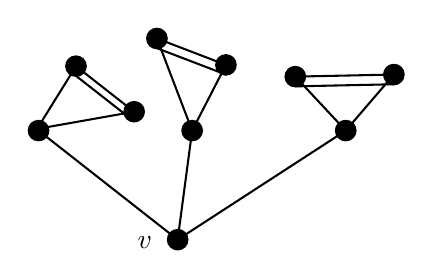
\begin{tikzpicture}[x=0.75pt,y=0.75pt,yscale=-1,xscale=1]
%uncomment if require: \path (0,300); %set diagram left start at 0, and has height of 300

%Shape: Ellipse [id:dp6157615359367345]
\draw  [fill={rgb, 255:red, 0; green, 0; blue, 0 }  ,fill opacity=1 ] (277.73,196.65) .. controls (280.34,196.64) and (282.46,198.73) .. (282.47,201.31) .. controls (282.49,203.9) and (280.39,206.01) .. (277.78,206.03) .. controls (275.17,206.04) and (273.05,203.96) .. (273.03,201.37) .. controls (273.02,198.78) and (275.12,196.67) .. (277.73,196.65) -- cycle ;
%Shape: Ellipse [id:dp386601276783894]
\draw  [fill={rgb, 255:red, 0; green, 0; blue, 0 }  ,fill opacity=1 ] (256.75,135.01) .. controls (259.36,134.99) and (261.48,137.08) .. (261.5,139.67) .. controls (261.51,142.26) and (259.41,144.37) .. (256.8,144.38) .. controls (254.19,144.4) and (252.07,142.31) .. (252.05,139.72) .. controls (252.04,137.13) and (254.14,135.02) .. (256.75,135.01) -- cycle ;
%Shape: Ellipse [id:dp07425790402378452]
\draw  [fill={rgb, 255:red, 0; green, 0; blue, 0 }  ,fill opacity=1 ] (284.7,144.09) .. controls (287.31,144.07) and (289.43,146.16) .. (289.45,148.75) .. controls (289.46,151.34) and (287.36,153.45) .. (284.75,153.46) .. controls (282.14,153.48) and (280.02,151.39) .. (280,148.8) .. controls (279.99,146.22) and (282.09,144.1) .. (284.7,144.09) -- cycle ;
%Shape: Ellipse [id:dp11996344977034723]
\draw  [fill={rgb, 255:red, 0; green, 0; blue, 0 }  ,fill opacity=1 ] (381.89,117.1) .. controls (384.5,117.08) and (386.62,119.17) .. (386.64,121.76) .. controls (386.65,124.35) and (384.55,126.46) .. (381.94,126.47) .. controls (379.33,126.49) and (377.21,124.4) .. (377.19,121.81) .. controls (377.18,119.22) and (379.28,117.11) .. (381.89,117.1) -- cycle ;
%Shape: Ellipse [id:dp28940132669054863]
\draw  [fill={rgb, 255:red, 0; green, 0; blue, 0 }  ,fill opacity=1 ] (358.7,144.09) .. controls (361.31,144.07) and (363.43,146.16) .. (363.45,148.75) .. controls (363.46,151.34) and (361.36,153.45) .. (358.75,153.46) .. controls (356.14,153.48) and (354.02,151.39) .. (354,148.8) .. controls (353.99,146.22) and (356.09,144.1) .. (358.7,144.09) -- cycle ;
%Shape: Ellipse [id:dp08349267618583034]
\draw  [fill={rgb, 255:red, 0; green, 0; blue, 0 }  ,fill opacity=1 ] (334.4,118.09) .. controls (337.01,118.08) and (339.13,120.16) .. (339.15,122.75) .. controls (339.16,125.34) and (337.06,127.45) .. (334.45,127.47) .. controls (331.84,127.48) and (329.72,125.4) .. (329.7,122.81) .. controls (329.69,120.22) and (331.79,118.11) .. (334.4,118.09) -- cycle ;
%Shape: Ellipse [id:dp9107142788834091]
\draw  [fill={rgb, 255:red, 0; green, 0; blue, 0 }  ,fill opacity=1 ] (228.74,113.06) .. controls (231.35,113.04) and (233.47,115.13) .. (233.49,117.72) .. controls (233.5,120.31) and (231.4,122.42) .. (228.79,122.43) .. controls (226.18,122.45) and (224.06,120.36) .. (224.04,117.77) .. controls (224.03,115.18) and (226.13,113.07) .. (228.74,113.06) -- cycle ;
%Shape: Ellipse [id:dp2920739309601139]
\draw  [fill={rgb, 255:red, 0; green, 0; blue, 0 }  ,fill opacity=1 ] (210.7,144.09) .. controls (213.31,144.07) and (215.43,146.16) .. (215.45,148.75) .. controls (215.46,151.34) and (213.36,153.45) .. (210.75,153.46) .. controls (208.14,153.48) and (206.02,151.39) .. (206,148.8) .. controls (205.99,146.22) and (208.09,144.1) .. (210.7,144.09) -- cycle ;
%Straight Lines [id:da4307039265371213]
\draw    (210.73,148.78) -- (277.75,201.34) ;
%Straight Lines [id:da48834390538516237]
\draw    (358.73,148.78) -- (277.75,201.34) ;
%Straight Lines [id:da09750211059585712]
\draw    (284.73,148.78) -- (277.75,201.34) ;
%Shape: Triangle [id:dp13555777212175668]
\draw   (228.76,117.75) -- (256.77,139.69) -- (210,147.98) -- cycle ;
%Shape: Triangle [id:dp0675108284609165]
\draw   (358.73,148.78) -- (334.43,122.78) -- (381.92,121.78) -- cycle ;
%Shape: Triangle [id:dp1406844325804908]
\draw   (301,117.13) -- (284.73,148.78) -- (267.77,104.4) -- cycle ;
%Shape: Ellipse [id:dp1365076686256248]
\draw  [fill={rgb, 255:red, 0; green, 0; blue, 0 }  ,fill opacity=1 ] (300.98,112.45) .. controls (303.59,112.43) and (305.71,114.52) .. (305.72,117.11) .. controls (305.74,119.69) and (303.64,121.8) .. (301.03,121.82) .. controls (298.42,121.83) and (296.3,119.75) .. (296.28,117.16) .. controls (296.27,114.57) and (298.37,112.46) .. (300.98,112.45) -- cycle ;
%Shape: Ellipse [id:dp24236222529832818]
\draw  [fill={rgb, 255:red, 0; green, 0; blue, 0 }  ,fill opacity=1 ] (267.75,99.72) .. controls (270.35,99.7) and (272.48,101.79) .. (272.49,104.38) .. controls (272.51,106.97) and (270.41,109.08) .. (267.8,109.09) .. controls (265.19,109.11) and (263.07,107.02) .. (263.05,104.43) .. controls (263.04,101.84) and (265.14,99.73) .. (267.75,99.72) -- cycle ;
%Straight Lines [id:da0057455971898583424]
\draw    (228.79,122.43) -- (256.8,144.38) ;
%Straight Lines [id:da5660132727377674]
\draw    (267.8,109.09) -- (301.03,121.82) ;
%Straight Lines [id:da17117560906894091]
\draw    (334.45,127.47) -- (381.94,126.47) ;

% Text Node
\draw (257,198.4) node [anchor=north west][inner sep=0.75pt]    {$v$};


\end{tikzpicture}
